\chapter{実装}
本章では,Stuguinシステムの実装について述べる.
はじめに実装環境について述べ,ついで学習記録モジュール,学習記録可視化モジュール,動機づけタイプ判定モジュール,内在化アプローチモジュールについて説明する.

\section{実装環境}
本節では,本システムにおける実装環境について説明する.本システムはiPhoneアプリケーションであり,実装言語にはSwiftを使用している.
サーバサイド兼データベースには,MBaaS (Mobile Backend as a Service)であるBack4App~\cite{back4app}を利用している.

\section{クライアント側実装}
クライアントはiPhoneアプリケーションであり,Swiftによって実装した.
学習記録モジュール,学習記録可視化モジュール,動機づけタイプ判定モジュール,内在化アプローチモジュールの4つのモジュールについて説明する.

\subsection{学習記録モジュール}
本節では学習記録モジュールについて説明する.
学習記録モジュールはユーザが学習した時間や教科,内容などを記録するモジュールである.記録の仕方は2種類あり,実際に測定する方法と時間を入力する方法である.
トップ画面の下タブにある``Study"ボタンを押すと,学習記録モジュールによって図~\ref{fig:study_alert}のようなUIAlertControllerが表示される.
このUIAlertControllerは,``勉強時間を計測する"と``勉強記録を手動で入力する"の2つの選択肢を持ったAction sheetである.

\begin{figure}[ht]
\begin{center}
\begin{tabular}{c}

	\begin{minipage}[b]{0.5\linewidth}
	\begin{center}
		\fbox{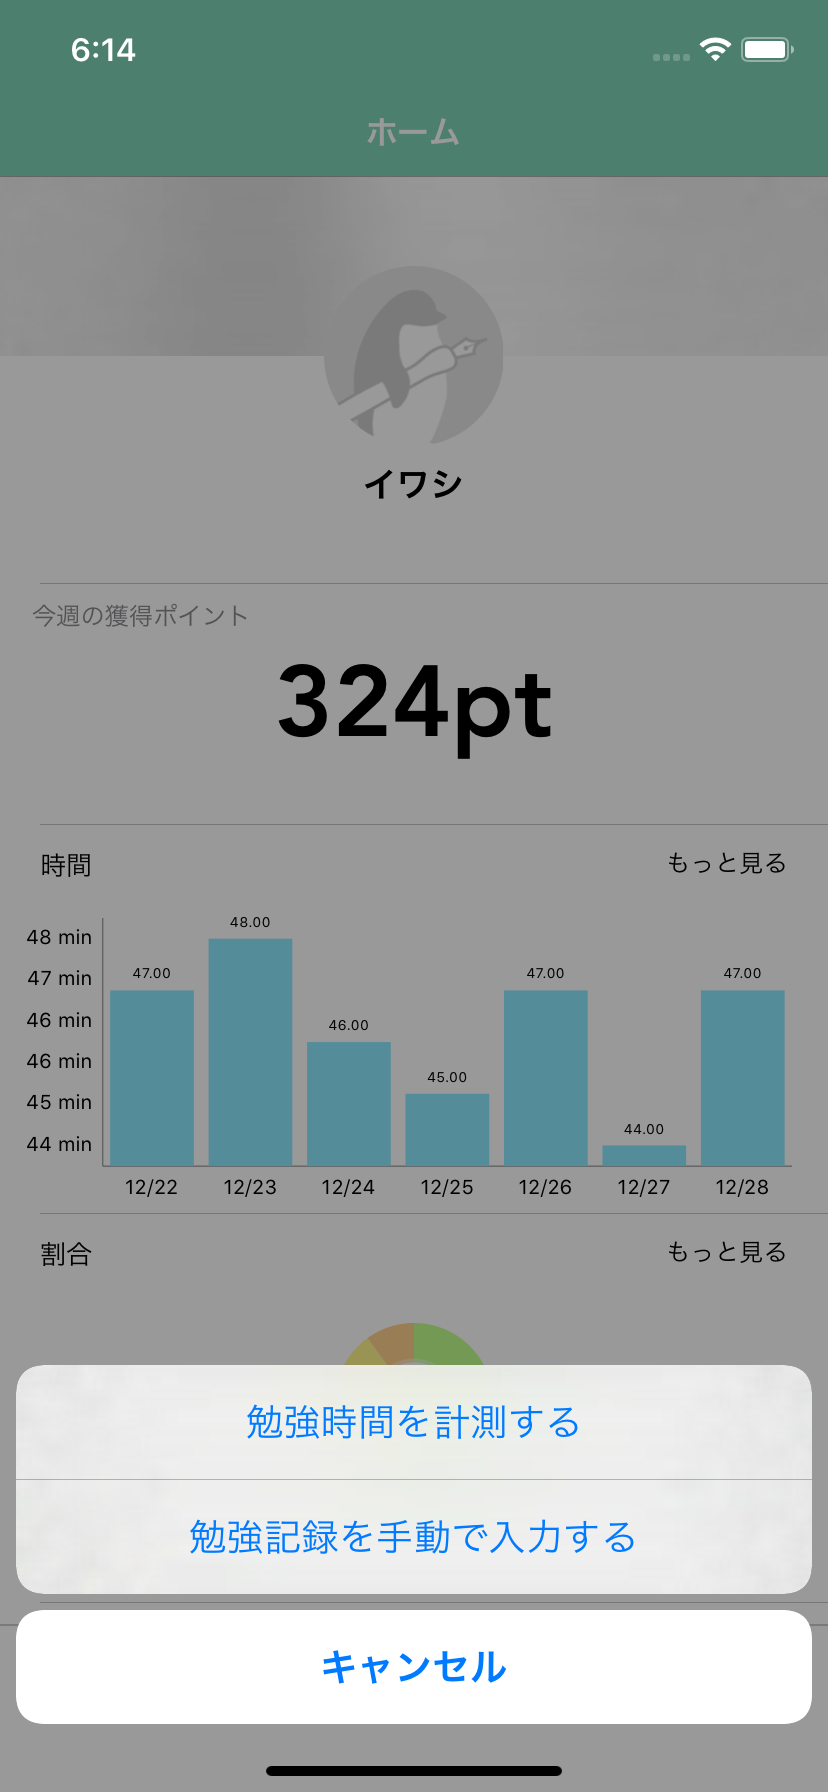
\includegraphics[width=5cm]{images/6/study_alert.png}}
		\caption{記録の仕方を選択させるAction sheet}
		\label{fig:study_alert}
	\end{center}
  	\end{minipage}

  	\begin{minipage}[b]{0.5\linewidth}
	\begin{center}
		\fbox{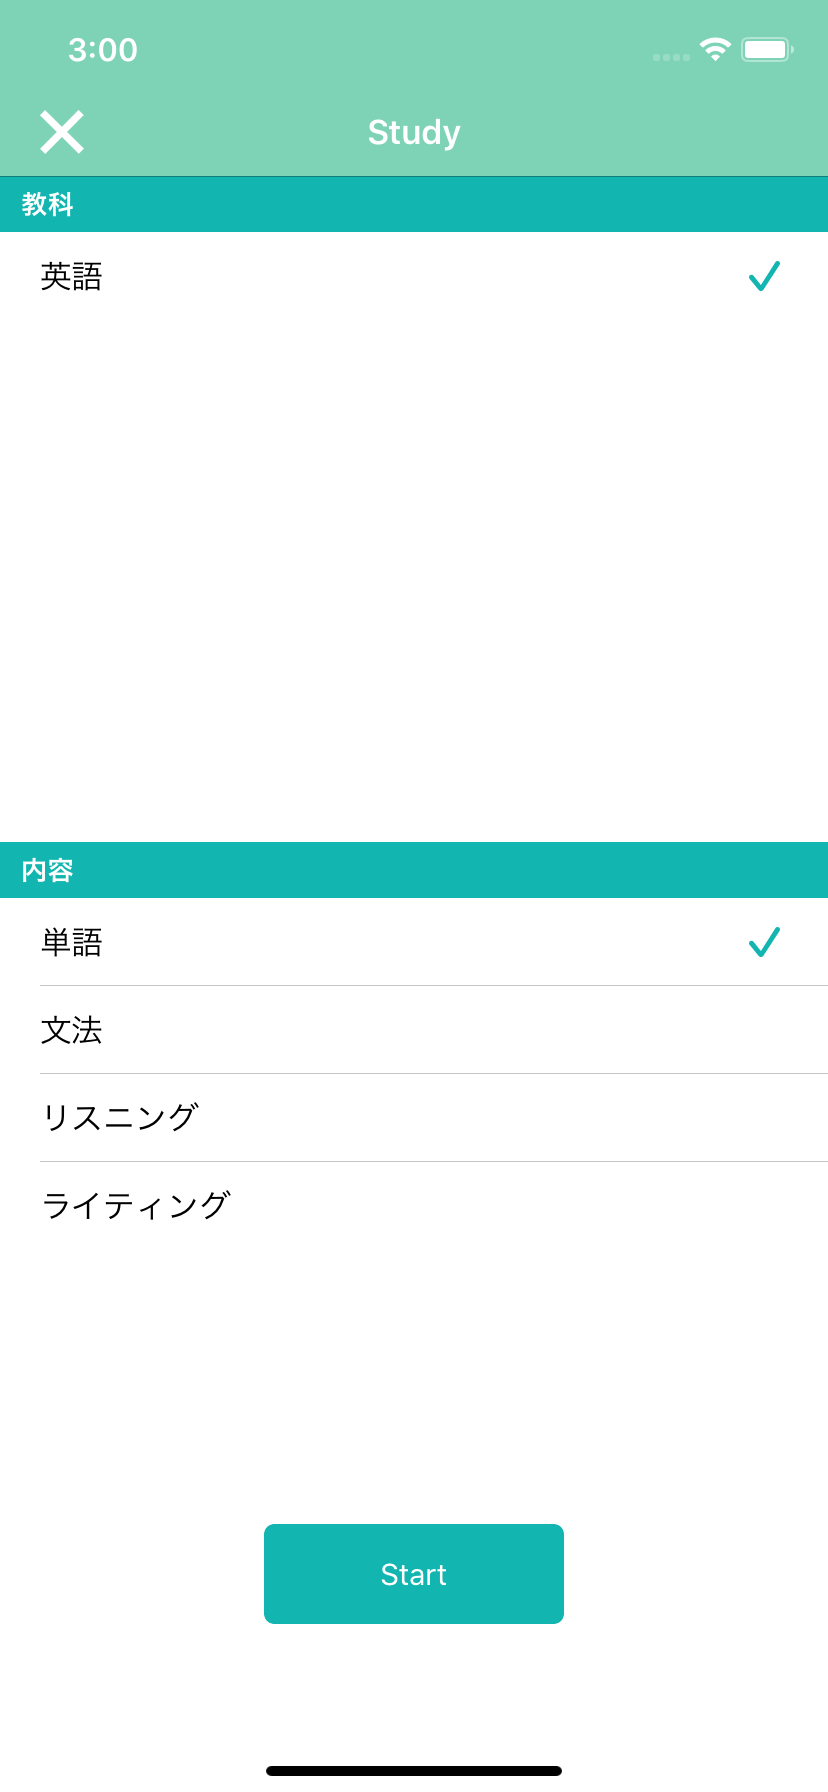
\includegraphics[width=5cm]{images/6/study_select.png}}
		\caption{教科及び内容の選択画面}
		\label{fig:study_select}
	\end{center}
  	\end{minipage}

  	\end{tabular}
  \end{center}
\end{figure}

``勉強時間を計測する"を選択すると,実際に測定する方法で学習を記録できる.
まず,これから学習する教科及び内容の選択画面が表示される.
この画面を図~\ref{fig:study_select}に示す.
ここに表示されている教科と内容は,端末内のUserDefaultsにString型の配列として保存されている.
表示には,教科と内容それぞれ別のUITableViewを用いている.
UITableView上のUITableViewCellをタップすると教科もしくは内容を選択することができる.
選択されているcellはaccessoryTypeにcheckmarkが指定され,右側にチェックマークが表示される.
画面下部の``Start"はUIButtonになっており,タップすると次の画面に選択された教科と内容をString型で渡し,その画面へ遷移する.

次の画面は時間を測定するものである.
この画面をインスタンス化する際,時間測定を担うViewModelが生成される.
このViewModelは生成されると同時にデバイス状態の監視を開始する.
デバイス状態とは,本アプリケーションが最前面に表示されているか否かや,iPhoneがロックされているかなどの状態を指す.
NotificationCenterを用いて,表~\ref{tb:NSNotification}の通知を監視することで現在のデバイス状態を判定する.

\begin{table}[htb]
\begin{center}
  \begin{tabular}{|l|l|} \hline
    NSNotification.Name & 通知受取時のデバイス状態 \\ \hline
    UIApplicationWillEnterForeground & 本アプリケーションがforegroundで実行されている \\
    UIApplicationDidEnterBackground & 本アプリケーションがbackgroundで実行されている \\
    UIApplicationProtectedDataDidBecomeAvailable & デバイスのロックが解除された \\ \hline
  \end{tabular}
  \caption{利用するNSNotification}
  \label{tb:NSNotification}
\end{center}
\end{table}

forgroundで実行されている状態とはすなわちアプリケーションが最前面に表示されている状態であり,backgroundで実行されている状態とはすなわちアプリケーションが閉じられiPhoneのホーム画面や他のアプリケーションなどが表示されている状態である.
測定中にアプリケーションが閉じられた場合は勉強が中断されたものとみなし記録を中断するが,iPhone自体がロックされた場合にはこの限りではない.
しかし,backgroundに移行したという通知だけではデバイスがロックされたかどうかは判定できない.
そのため,UIApplicationProtectedDataDidBecomeAvailableという通知を用いる.この通知はアプリケーションの保護データにアクセス可能となった時に送られるものであり,それはほぼロック解除のタイミングである.
したがって,UIApplicationDidEnterBackgroundの通知後,UIApplicationWillEnterForegroundと同時にUIApplicationProtectedDataDidBecomeAvailableの通知を受け取った場合には,先のbackground移行はデバイスロックによるものであったと判定できる.
また,UIApplicationDidEnterBackgroundの通知後,UIApplicationWillEnterForegroundによる通知のみを受け取った場合には本アプリケーションが閉じられホーム画面や他のアプリケーションが使用されたと判定できる.

Appleの公式ドキュメント~\cite{apple}にはUIApplicationProtectedDataDidBecomeAvailableがロック解除時に通知されるという記載はないが,現在この他にデバイスロックを検知するAPIが提供されていないため,暫定的にこの措置をとった.

ViewModelは時間の計測中はデバイス状態の監視を続け,アプリケーションがbackgroundに遷移した際は計測を一時停止する.
次にforegroundに戻ってきた際,UIApplicationProtectedDataDidBecomeAvailableによる通知を受け取っていれば計測を再開,そうでない場合には計測を終了する.
デバイス状態の監視による判定で計測を終了した場合は,中断された学習として記録される.

\begin{figure}[htb]
	\begin{center}
	\fbox{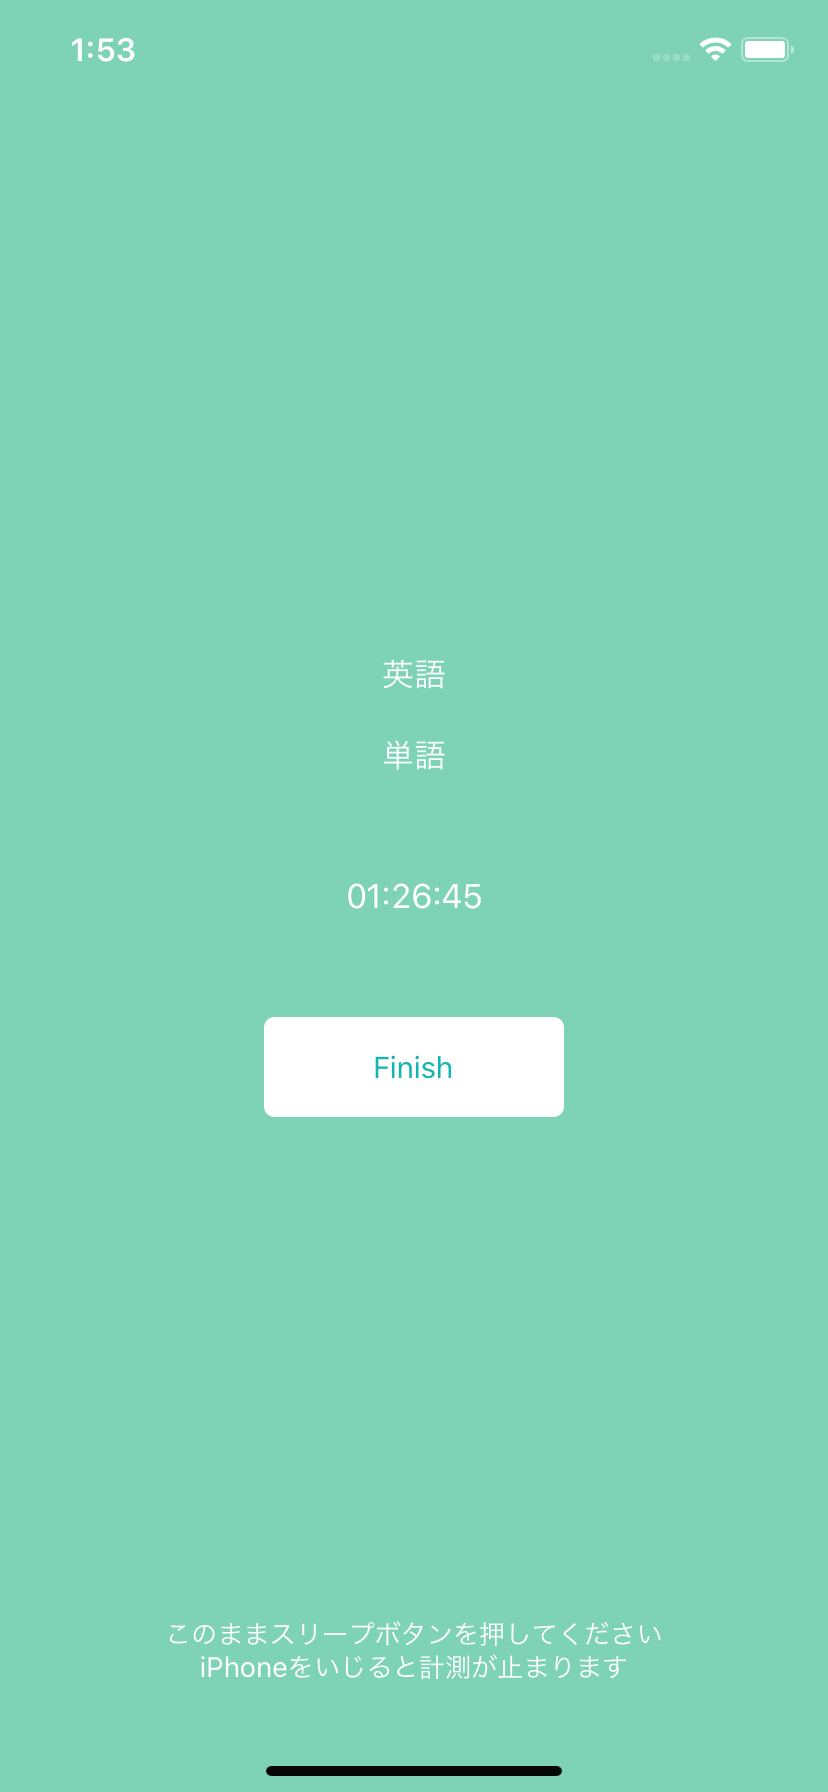
\includegraphics[width=5cm]{images/6/measure.png}}
	\caption{学習時間計測画面}
	\label{fig:measure}
	\end{center}
\end{figure}

学習時間測定中の画面を図~\ref{fig:measure}に示す.
本画面には3つのUILabelと1つのUIButtonが存在する.
上2つのUILabelには,前の画面から渡された教科と内容が表示される.
3つ目のUILabelには,本画面に遷移してきてからの経過時間が``hh:mm:ss"の書式で表示される.
画面下部の``Finish"と表示されたUIButtonをタップすると,時間の測定が終了し,次の画面へ遷移する.
この時,学習した教科,内容,学習時間及び学習が中断されたかどうかの情報が同時に渡される.

\begin{figure}[htb]
\begin{center}
\begin{tabular}{c}

	\begin{minipage}[b]{0.5\linewidth}
	\begin{center}
		\fbox{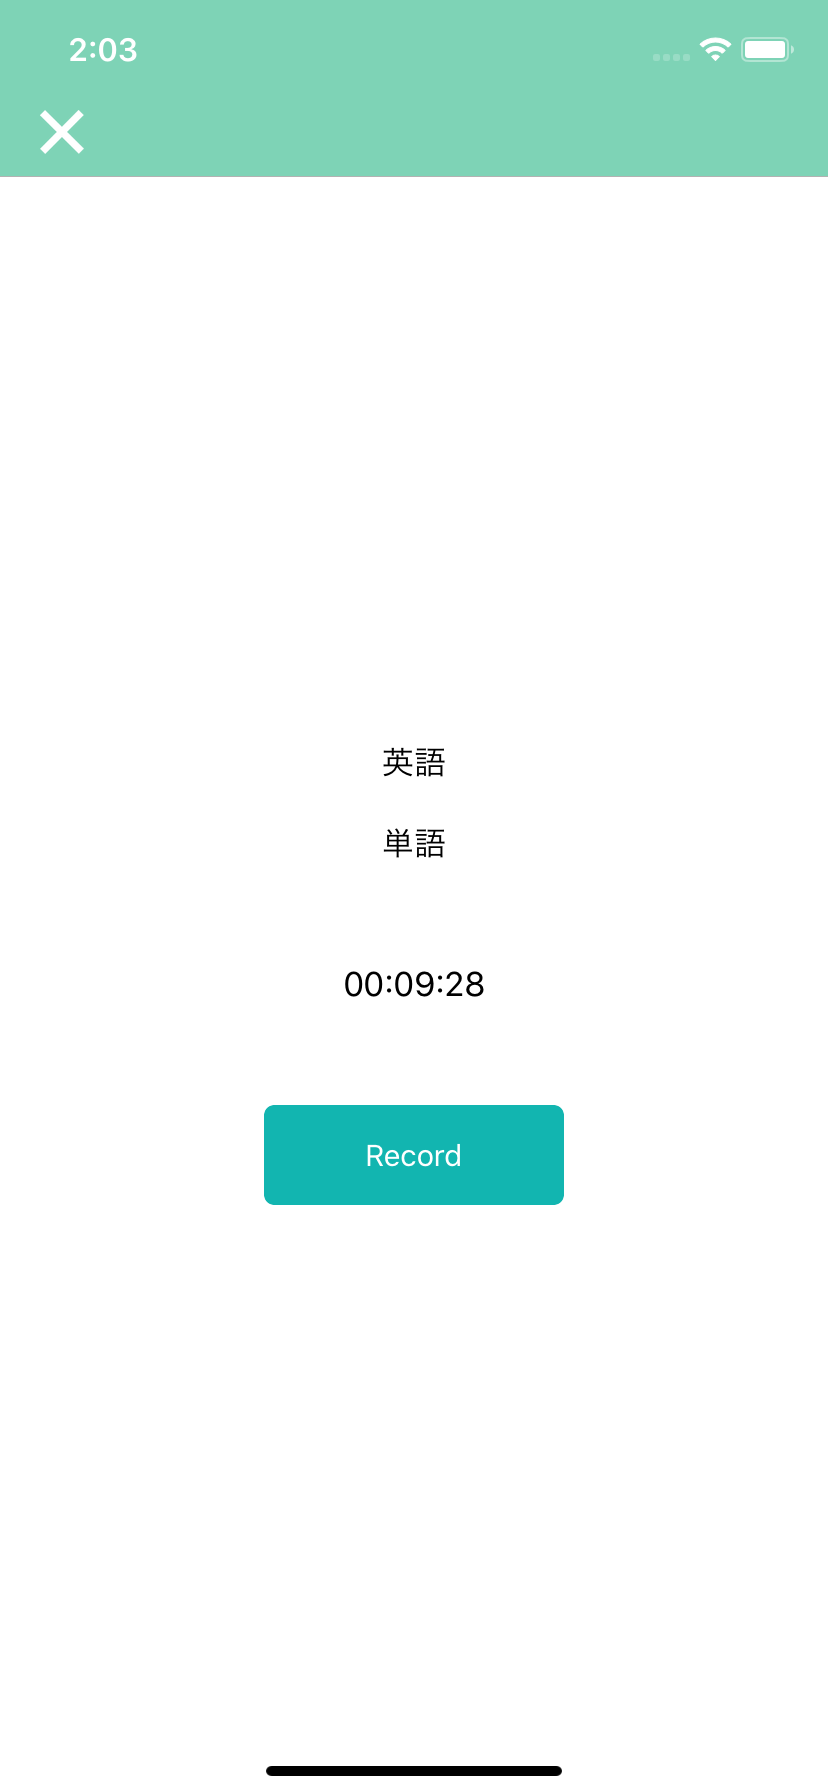
\includegraphics[width=5cm]{images/6/finish.png}}
		\caption{学習時間計測終了画面}
		\label{fig:finish}
	\end{center}
  	\end{minipage}

  	\begin{minipage}[b]{0.5\linewidth}
	\begin{center}
		\fbox{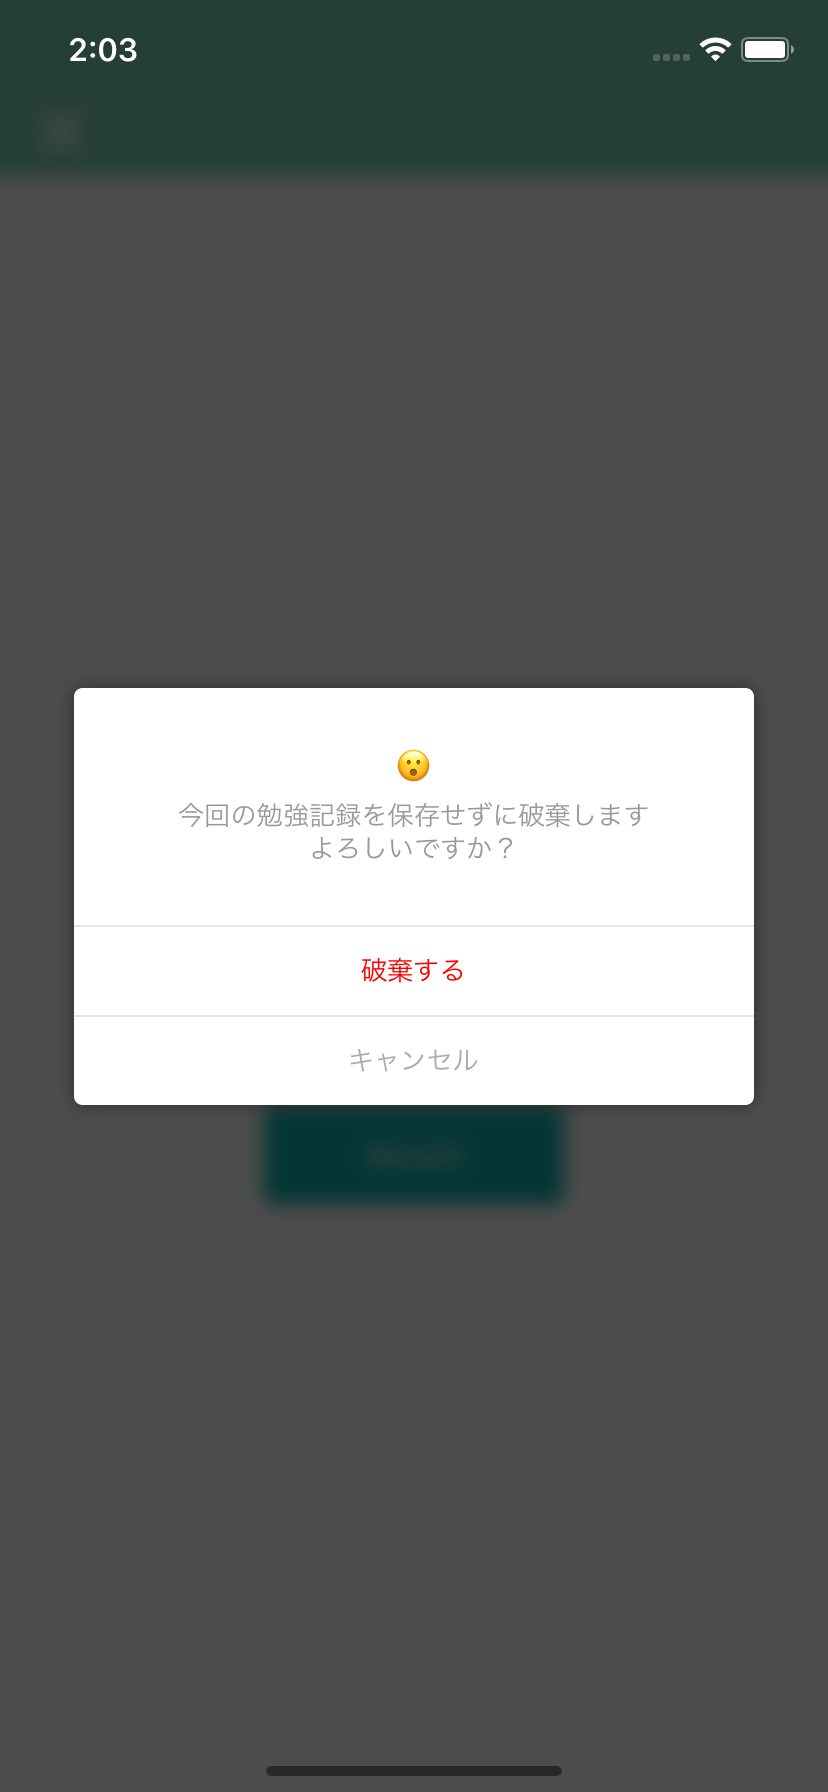
\includegraphics[width=5cm]{images/6/study_discard.png}}
		\caption{学習記録を破棄する際の確認アラート}
		\label{fig:study_discard}
	\end{center}
  	\end{minipage}

\end{tabular}
\end{center}
\end{figure}

次の画面では学習した教科,内容及び学習時間をUILabelに表示する.
この画面を図~\ref{fig:finish}に示す.
画面下部に``Record"と表示されたUIButtonが設置されており,これをタップすると学習記録がサーバに送られ,学習記録モジュールを終了する.
左上のバツ印となっているUIButtonをタップすると,図~\ref{fig:study_discard}のように``今回の学習記録を破棄してよいか"という旨のUIAlertControllerが表示される.
ユーザが``破棄する"を洗濯した場合には,学習記録をサーバに送らずに学習記録モジュールを終了する.

学習記録モジュールが最初に表示するAction sheet(図~\ref{fig:study_select})において``勉強記録を手動で入力する"を選択すると,図~\ref{fig:study_input}のような入力画面が表示される.
この画面にはUITableViewが設置されており,``日時",``教科",``内容",``勉強時間"の4項目からなる.

\begin{figure}[hb]
	\begin{center}
	\fbox{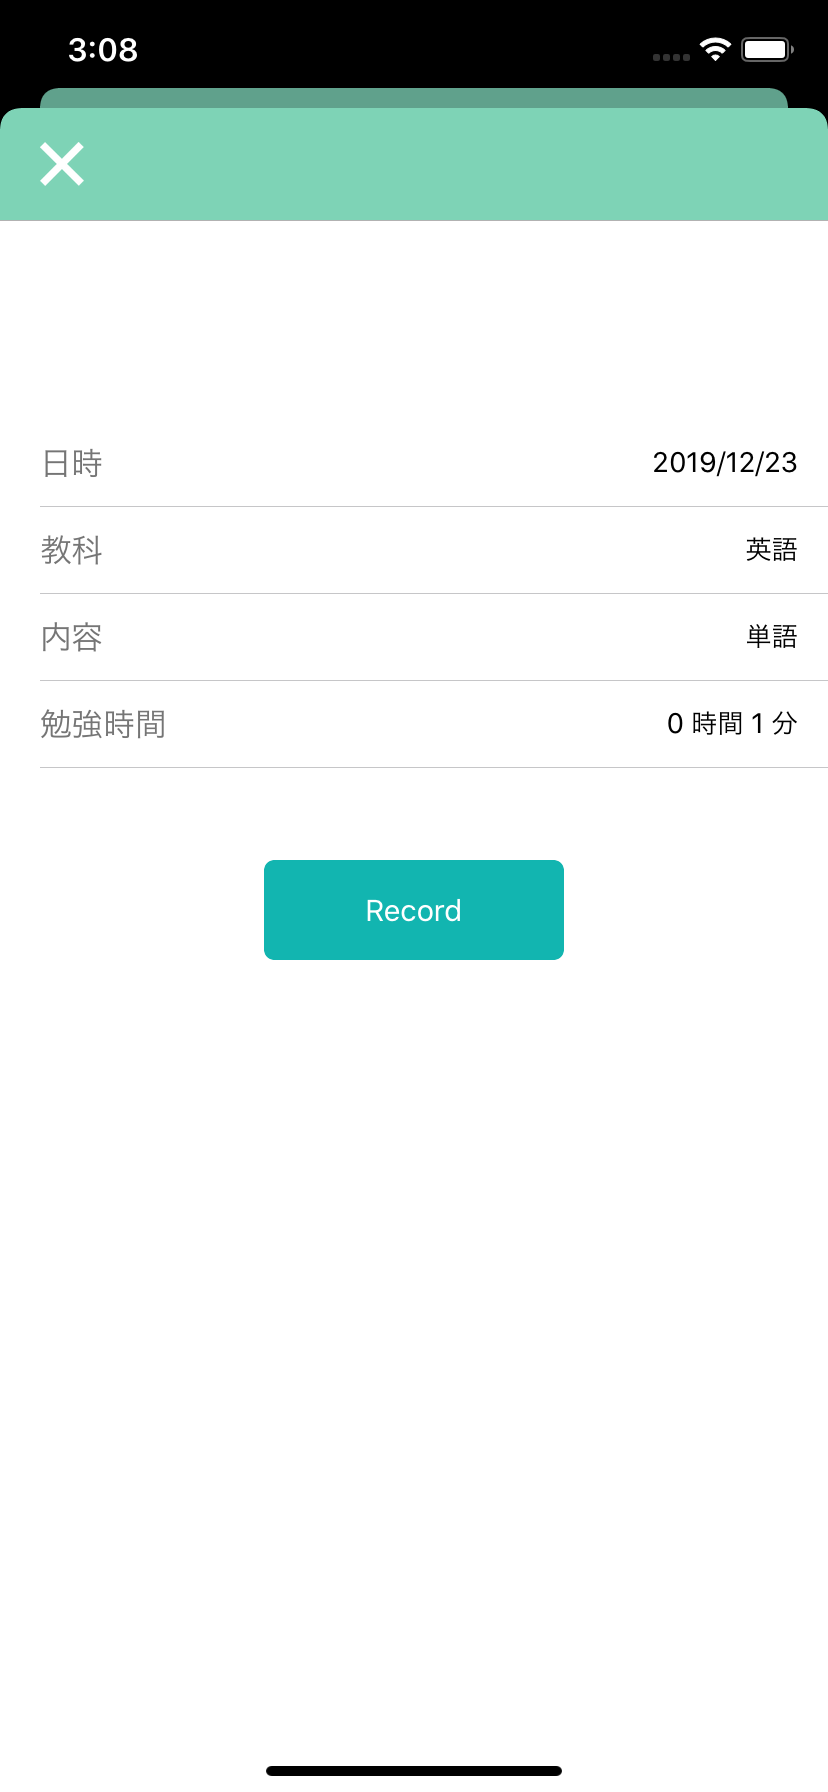
\includegraphics[width=5cm]{images/6/study_input.png}}
	\caption{学習記録入力画面}
	\label{fig:study_input}
	\end{center}
\end{figure}

一番上の``日時"をタップすると,日付を選択できるUIDatePickerViewが出現する.
これより学習を行った日付を選択する.
本日より後の日付は無効化されており選択することができない.
``教科"もしくは``内容"をタップすると,UIPickerViewが出現するので,これより学習した教科もしくは内容を選択する.
``勉強時間"をタップすると,時間と分を指定することができるUIDatePickerViewが出現するので,これより学習した時間を指定する.
1分未満の学習時間は指定することができない.

画面下部にある``Record"と表示されたUIButtonを押すと,入力した学習記録がサーバに送られ,学習記録モジュールを終了する.
左上のバツ印となっているUIButtonをタップすると,学習記録をサーバに送らずに学習記録モジュールを終了する.

サーバに送られる学習記録の値は表~\ref{tb:study_record}の通りである.

\begin{table}[htb]
\begin{center}
  \begin{tabular}{|l|l|} \hline
    サーバに送る値 & 型 \\ \hline
    ユーザID & PFUser型(サーバ指定のユーザ型) \\
    学習日時 & Date型 \\
    教科 & String型 \\ 
    内容 & String型 \\ 
	学習時間(秒) & Int型 \\ 
	学習が中断されたか否か & Bool型 \\ 
	記入による記録か否か & Bool型 \\  \hline
  \end{tabular}
  \caption{学習記録の値とその型}
  \label{tb:study_record}
\end{center}
\end{table}

\subsection{学習記録可視化モジュール}
学習記録可視化モジュールでは,前項の学習記録モジュールにて保存した学習記録を可視化する.

\begin{figure}[ht]
	\begin{center}
	\fbox{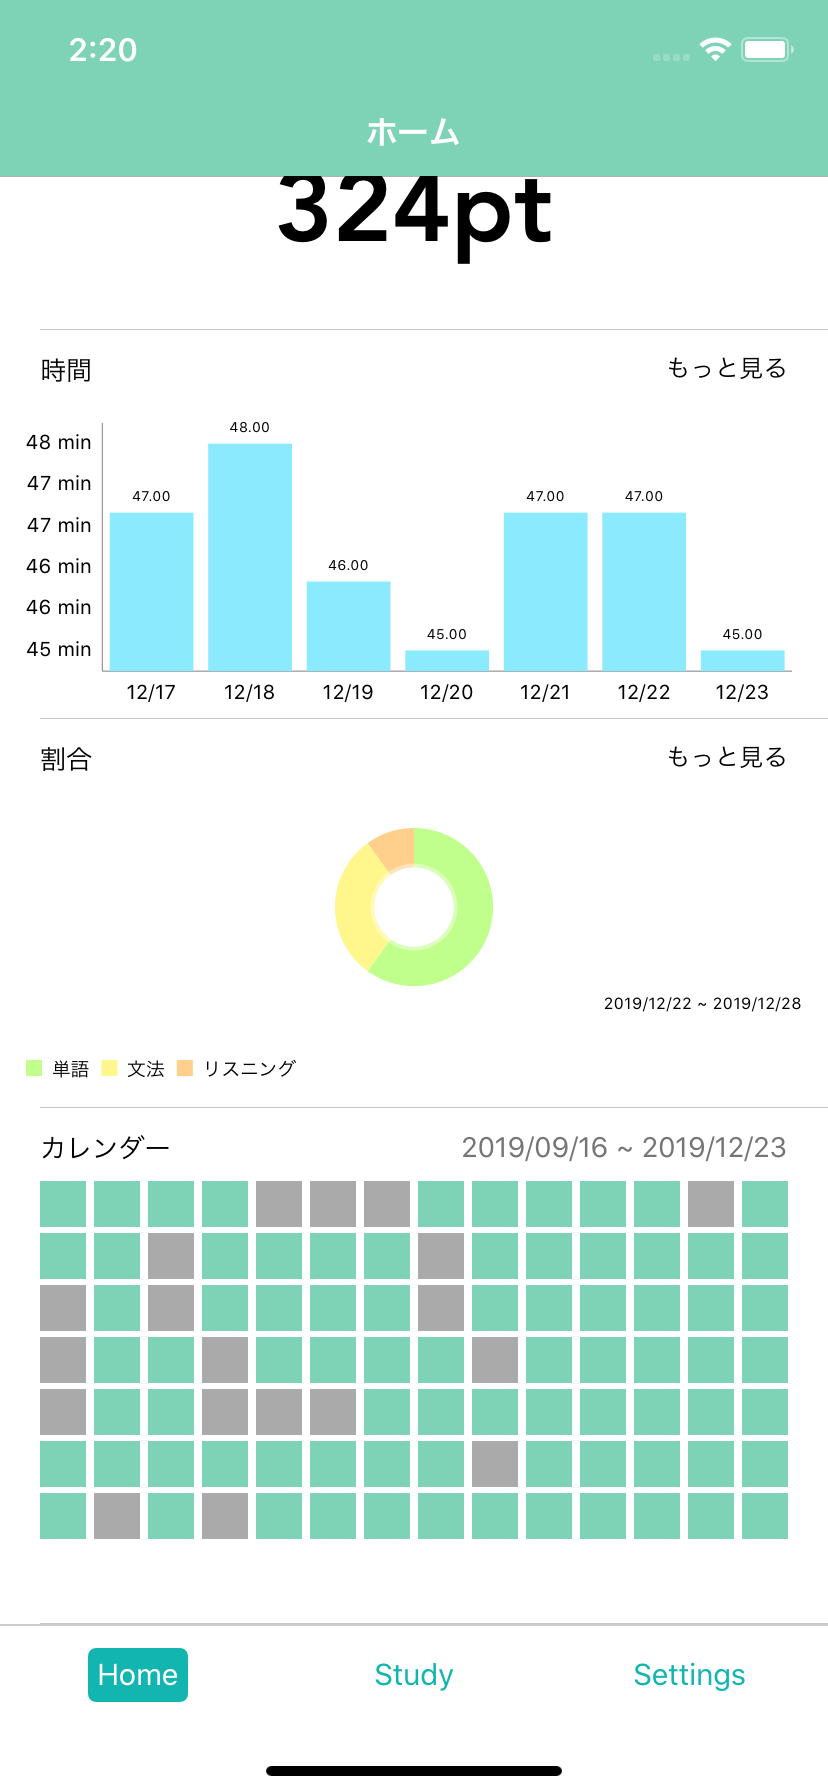
\includegraphics[width=5cm]{images/6/outline.png}}
	\caption{トップ画面に表示される学習記録の概要}
	\label{fig:outline}
	\end{center}
\end{figure}

まず,トップ画面の生成時にローカルのデータベースより過去14週間分の学習記録が配列として読み込まれる.
ここから直近1週間分の学習記録を取得し,1日ごとの合計学習時間を計算し,keyが日付,valueが合計学習時間からなるDictionary型の配列を生成する.
この配列を,iOS用のグラフ描画ライブラリである``Charts"に渡し,棒グラフとしてトップ画面に表示する.

次に,同じく直近1週間分の学習記録から,教科ごとの学習時間の合計を計算し,学習時間に対する教科の割合を算出する.
この結果から,keyが日付,valueが合計学習時間からなるDictionary型の配列を生成する.
この配列を,``Charts"ライブラリに渡し,円グラフとしてトップ画面に表示する.

最後に過去14週間分の学習記録より,学習を記録した日付をDate型の配列として生成する.
続いて,7*14個分の要素からなるUICollectionViewを作る.
右下のセルを今日,その1つ左のセルを昨日とみなしそれぞれ日付を割り当て,先ほど生成したDate型の配列に含まれている日付のセルに色付けを行う.
これにより,カレンダー表記の可視化を行う.

\begin{figure}[hb]
\begin{center}
\begin{tabular}{c}
  	\begin{minipage}[b]{0.5\linewidth}
	\begin{center}
		\fbox{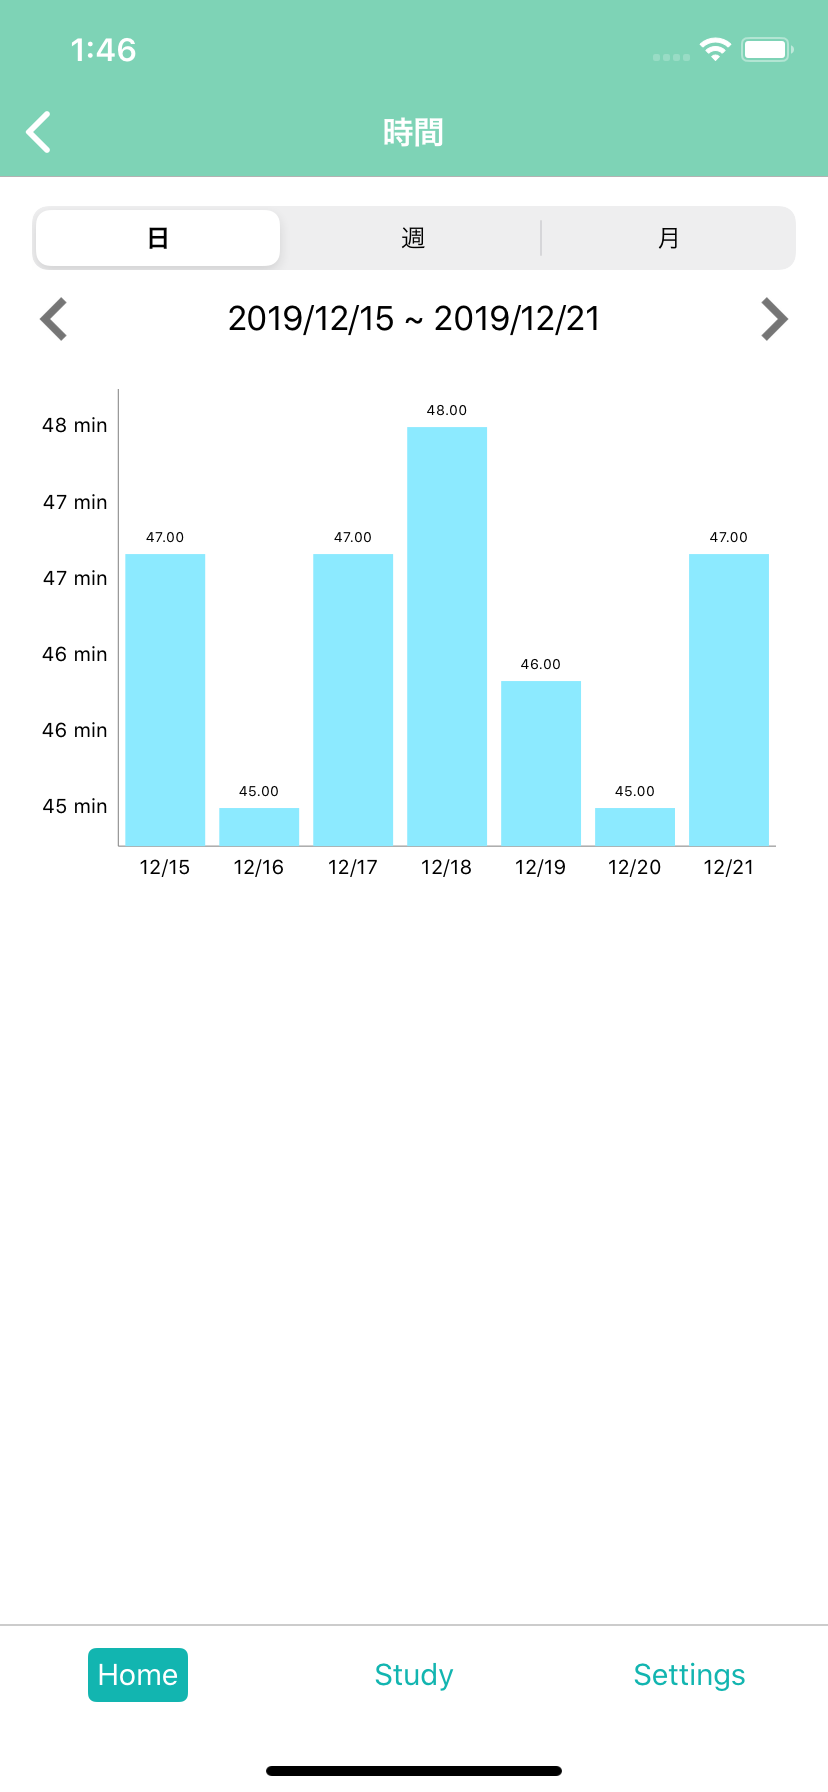
\includegraphics[width=5cm]{images/6/time_detail.png}}
		\caption{学習時間の詳細画面}
		\label{fig:time_detail}
	\end{center}
  	\end{minipage}

  	\begin{minipage}[b]{0.5\linewidth}
	\begin{center}
		\fbox{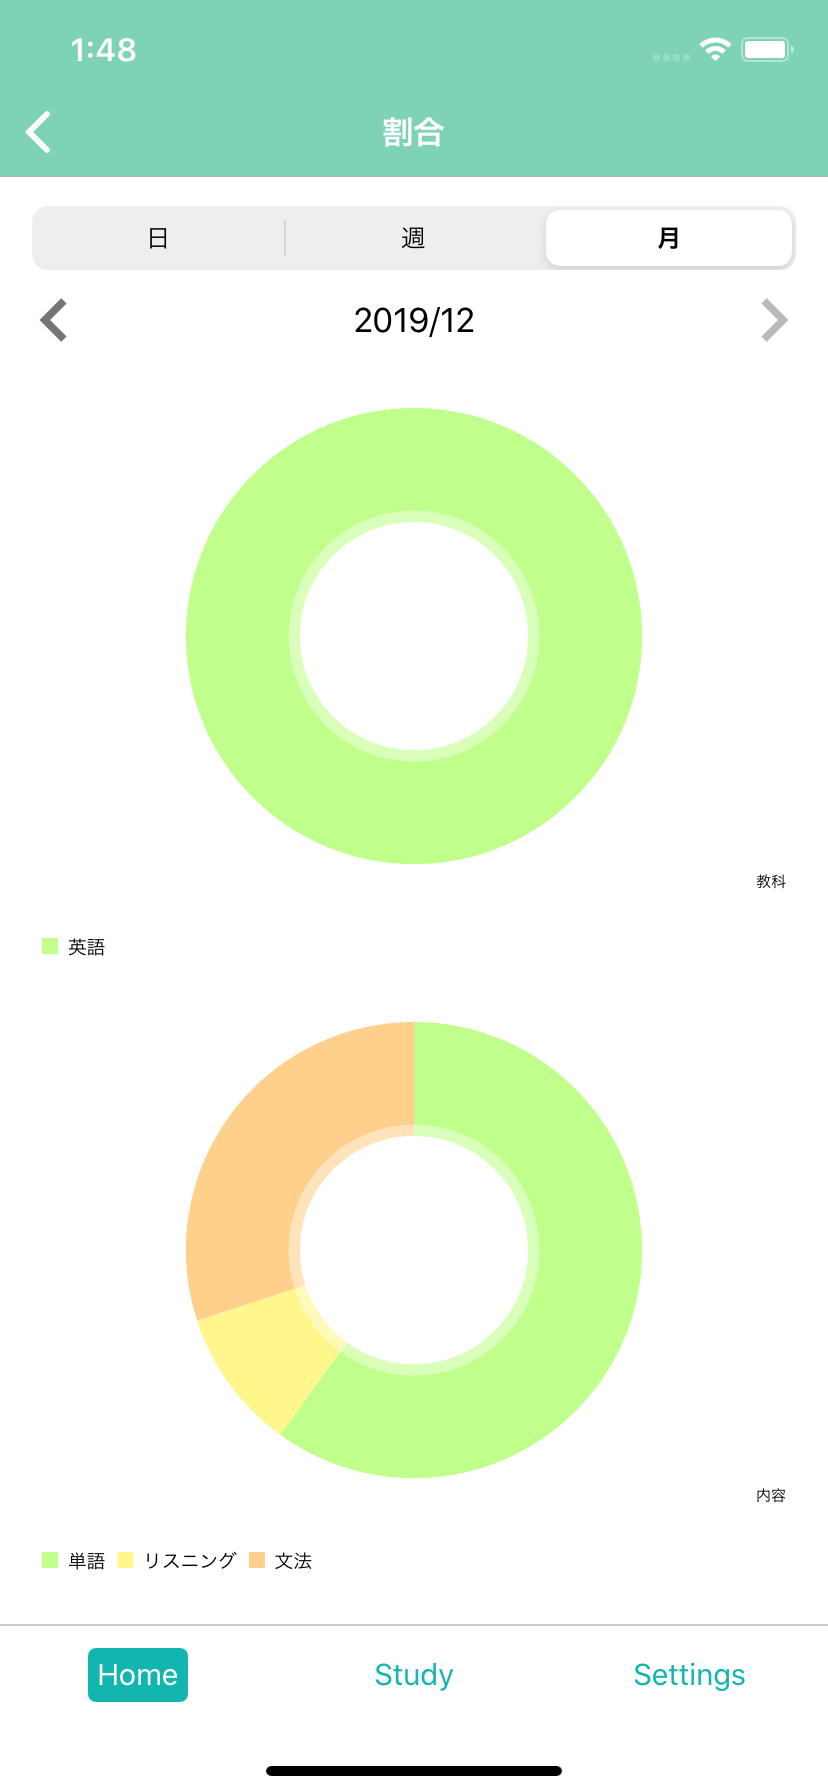
\includegraphics[width=5cm]{images/6/ratio_detail.png}}
		\caption{学習した教科および内容の詳細画面}
		\label{fig:ratio_detail}
	\end{center}
  	\end{minipage}

  	\end{tabular}
  \end{center}
\end{figure}

棒グラフ,円グラフ,カレンダーの3つを学習記録の概要として図~\ref{fig:outline}のようにトップ画面に表示する.
棒グラフをタップすると,学習時間の詳細を閲覧できる画面に遷移する.
この画面を図~\ref{fig:time_detail}に示す.
この画面にはUISegmentedControlが置かれており,``日",``週",``月"を選択できる.
その下には日付が表示されたUILabelと日付を変更することのできるUIButtonが置かれている.
これらを切り替えることにより,日ごと,週ごと,月ごとの合計学習時間を閲覧することができる.

円グラフをタップすると,学習した教科と内容の割合を詳しく閲覧できる画面に遷移する.
この画面を図~\ref{fig:ratio_detail}に示す.
この画面にもUISegmentedControlが設置されており,``日",``週",``月"を選択できる.
その下には日付が表示されたUILabelと日付を変更することのできるUIButtonが置かれている.
これらを切り替えることにより,日ごと,週ごと,月ごとの教科の割合及び内容の割合を閲覧することができる.

\subsection{動機づけタイプ判定モジュール}

動機づけタイプ判定モジュールは,1週間ごとにアンケートを要求し,その結果から動機づけタイプを判定するモジュールである.
トップ画面が生成されると同時にサーバと通信して,新たにアンケートを要求する必要があるかをチェックする.
その必要があった場合には,図~\ref{fig:questionnaire_alert}のようにアンケートを要求するUIAlertControllerを表示する.

\begin{figure}[ht]
\begin{center}
\begin{tabular}{c}

	\begin{minipage}[b]{0.5\linewidth}
	\begin{center}
		\fbox{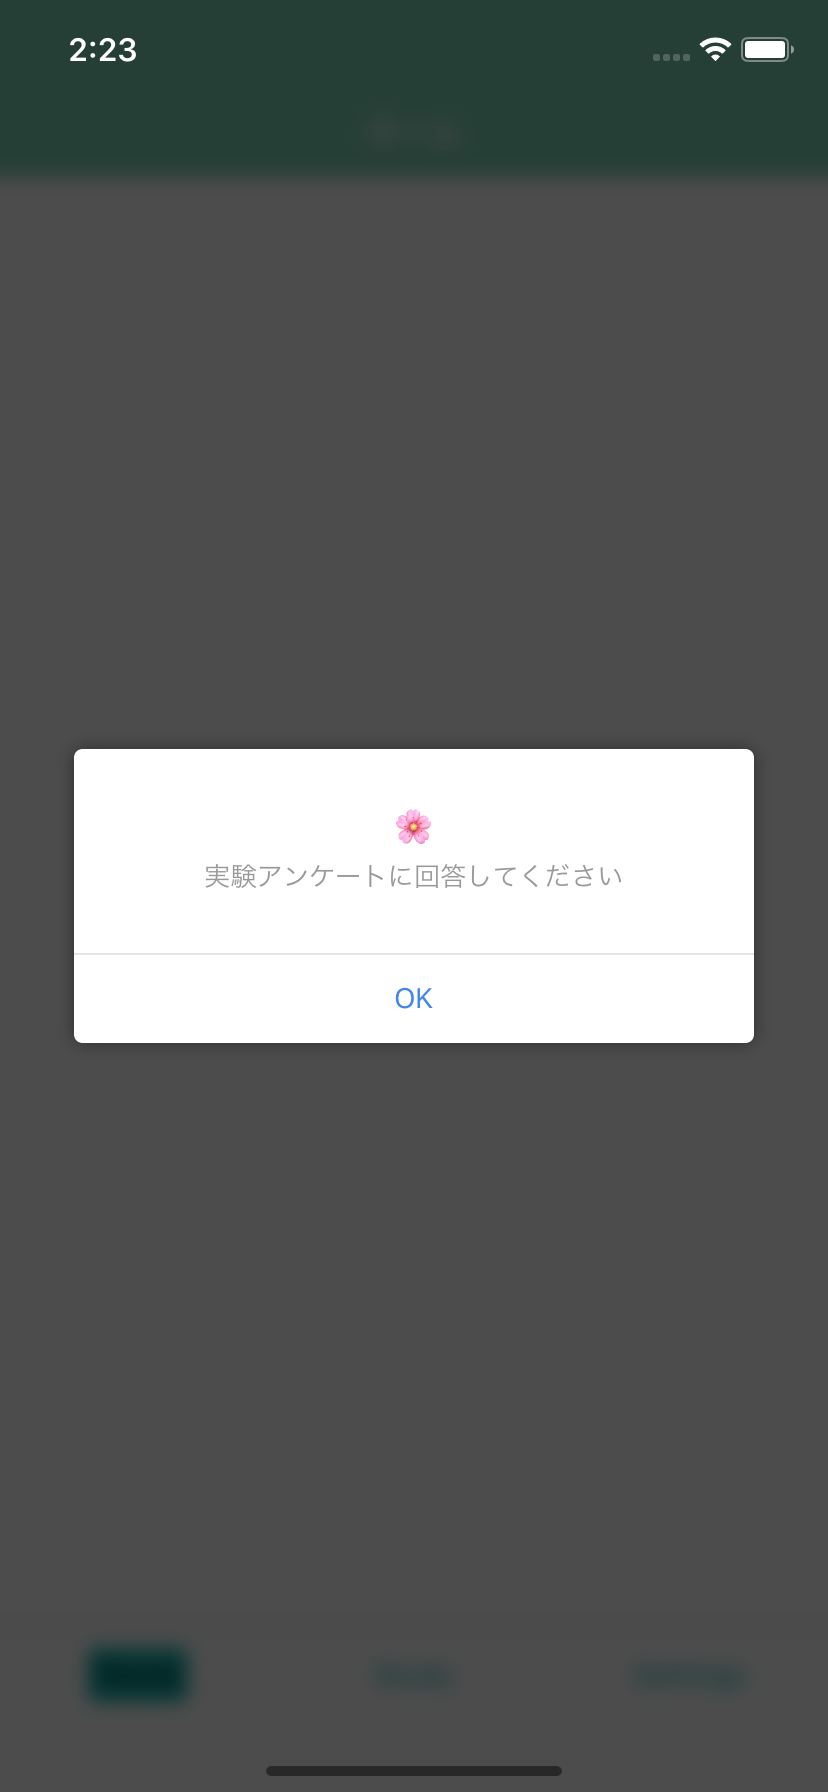
\includegraphics[width=5cm]{images/6/questionnaire_alert.png}}
		\caption{アンケート要求アラート}
		\label{fig:questionnaire_alert}
	\end{center}
  	\end{minipage}

  	\begin{minipage}[b]{0.5\linewidth}
	\begin{center}
		\fbox{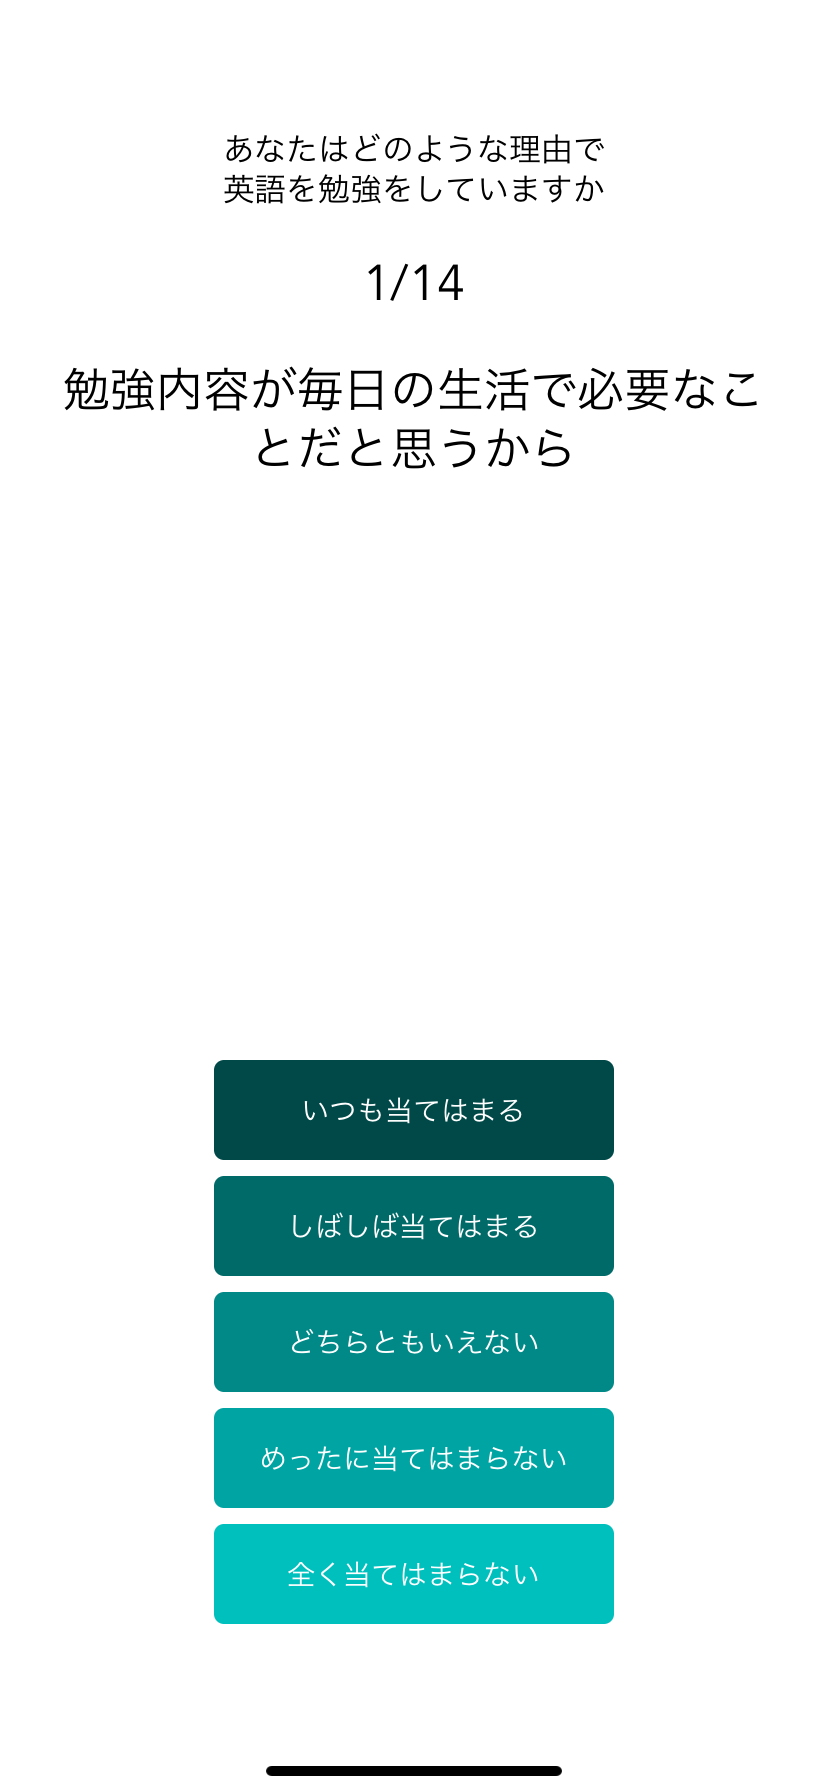
\includegraphics[width=5cm]{images/6/questionnaire.png}}
		\caption{アンケート回答画面}
		\label{fig:questionnaire}
	\end{center}
  	\end{minipage}

\end{tabular}
\end{center}
\end{figure}

このアラートは拒否することができないため,アンケートを回答しなければStuguinシステムの他の機能は利用することができない.
アラートを許可すると,アンケート画面に遷移する.
この画面には,図~\ref{fig:questionnaire}に見られるように,質問文を表示するUILabelと,``いつも当てはまる",``しばしば当てはまる",``どちらともいえない",``めったに当てはまらない",``全く当てはまらない"の5つのUIButtonが設置されている.
質問文はString型として配列に格納されており,5つのUIButtonのうちどれか1つを選択すると,UILabelに次の質問文が表示される.
回答するごとに,``いつも当てはまる"を4,``しばしば当てはまる"を3,``どちらともいえない"を2,``めったに当てはまらない"を1,``全く当てはまらない"を0として,対応する動機づけタイプの合計点数に足していく.
最も点数が大きかった動機づけタイプを,ユーザが現在抱く動機づけタイプと判定する.
判定された動機づけタイプは,デバイスのローカルデータベースとサーバ上のデータベースに保存される.

\subsection{内在化アプローチモジュール}
内在化アプローチモジュールは,前項の動機づけタイプ判定モジュールにて判定された動機づけタイプに応じて,トップ画面の一番上に表示する機能を切り替えるモジュールである.
機能は3種類あり,外的調整に向けた``ポイント機能",取り入れ的調整に向けた``ランキング機能",同一化的調整に向けた``目標設定機能"からなる.

``ポイント機能"は外的調整による動機づけを抱くユーザに向けた機能である.
現在の週の学習時間を,1分1ポイントとして換算して換算し,トップ画面に表示する.
この機能が表示された際のトップ画面を図~\ref{fig:top_point}に示す.

``ランキング機能"は取り入れ的調整による動機づけを抱くユーザに向けた機能である.
現在の週の総学習時間を他ユーザの分も取得し,ランキング形式で表示する.
この機能が表示された際のトップ画面を図~\ref{fig:top_ranking}に示す.

``目標設定機能"は同一化的調整による動機づけを抱くユーザに向けた機能である.
この機能に切り替わった時,はじめにUIAlertControllerが表示される.
この時の画面を図~\ref{fig:goal_alert}に示す.
このアラートはUITextFieldを持っており,ユーザは今週の目標学習時間を設定するよう要求される.
入力をしないとこのアラートを閉じることができないため,ユーザは必ず目標を設定する必要がある.
ユーザによって入力された数値は,ローカルのデータベース及びサーバ上のデータベースに保存する.
これ以降は,図~\ref{fig:top_goal}目標の達成割合をトップ画面に表示する.

\begin{figure}[ht]
\begin{center}
\begin{tabular}{c}

	\begin{minipage}[b]{0.5\linewidth}
	\begin{center}
		\fbox{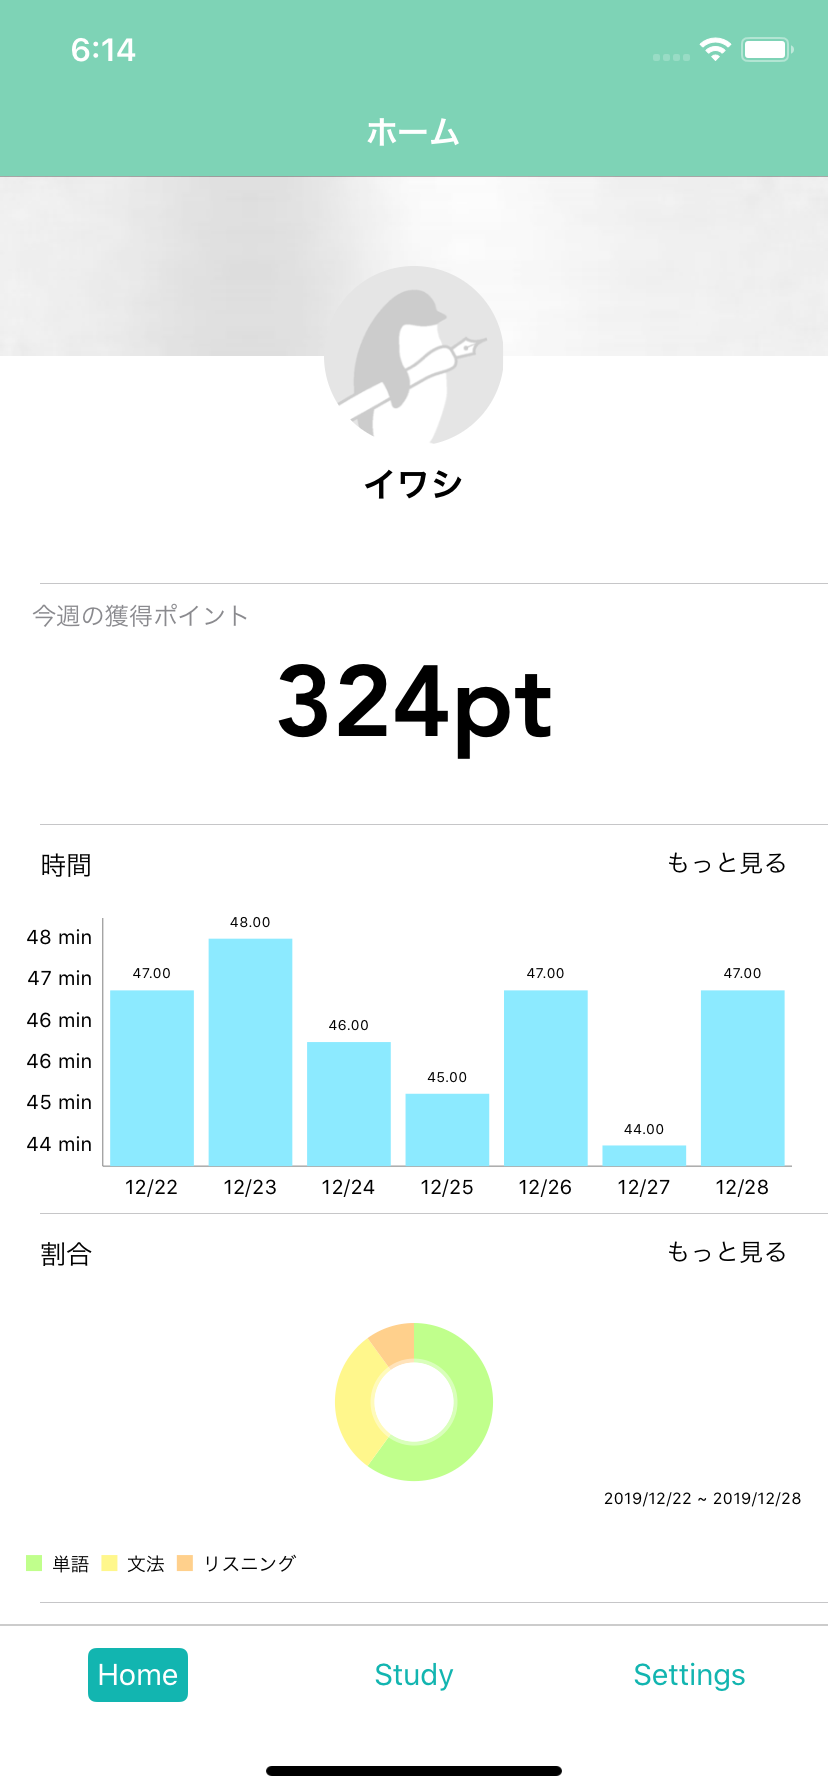
\includegraphics[width=5cm]{images/6/top_point.png}}
		\caption{ポイント機能}
		\label{fig:top_point}
	\end{center}
  	\end{minipage}

  	\begin{minipage}[b]{0.5\linewidth}
	\begin{center}
		\fbox{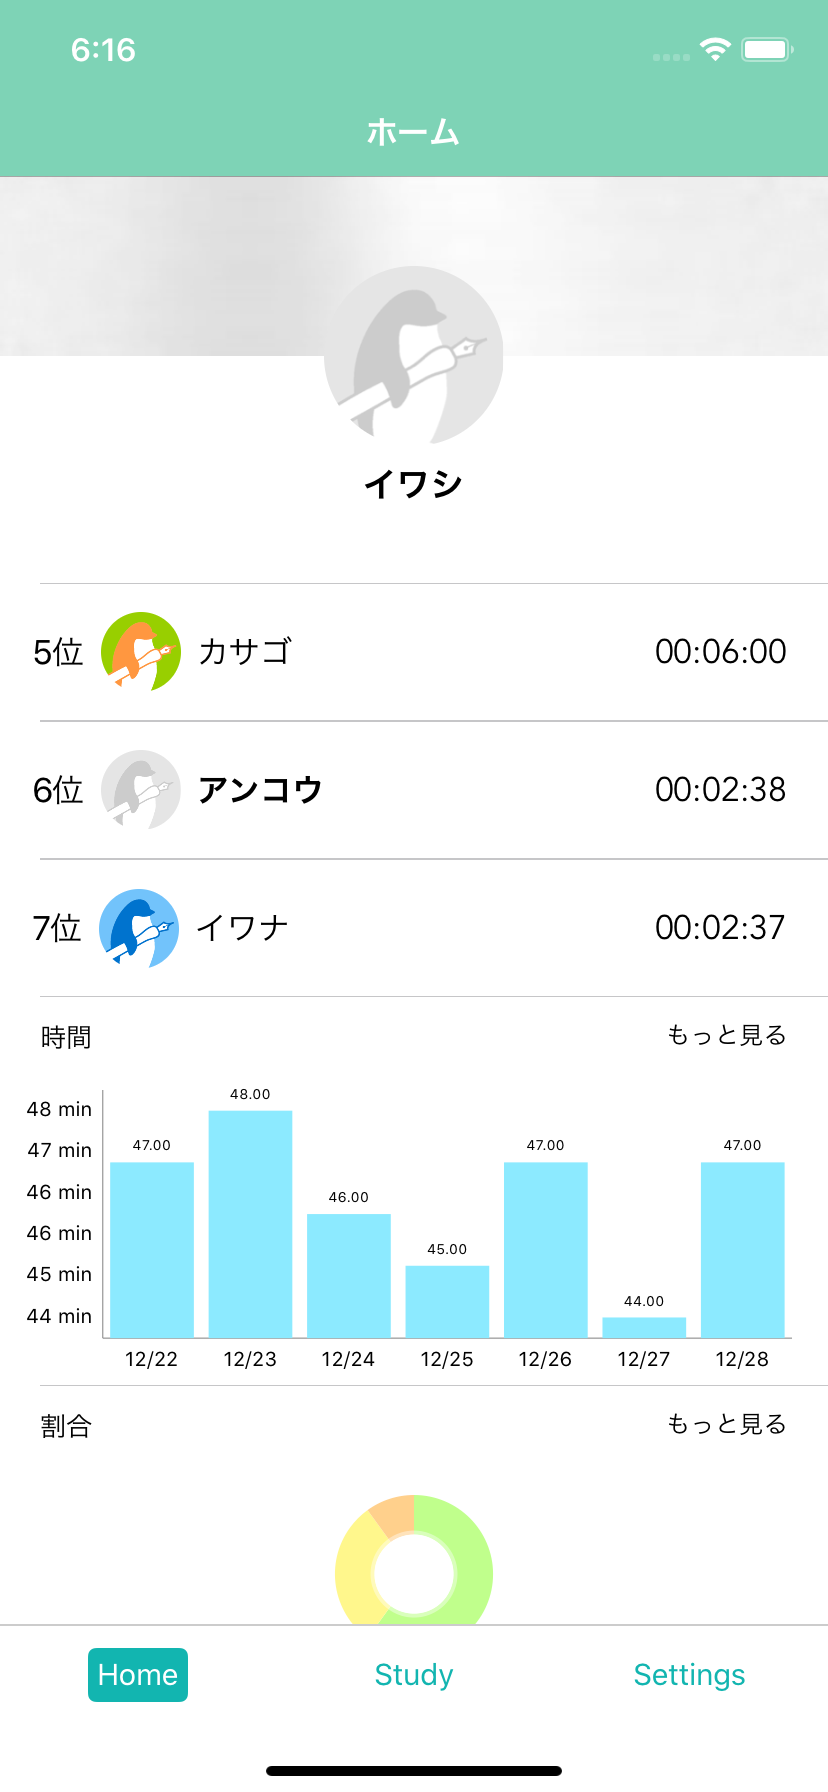
\includegraphics[width=5cm]{images/6/top_ranking.png}}
		\caption{ランキング機能}
		\label{fig:top_ranking}
	\end{center}
  	\end{minipage}

  	\\

  	\begin{minipage}[b]{0.5\linewidth}
	\begin{center}
		\fbox{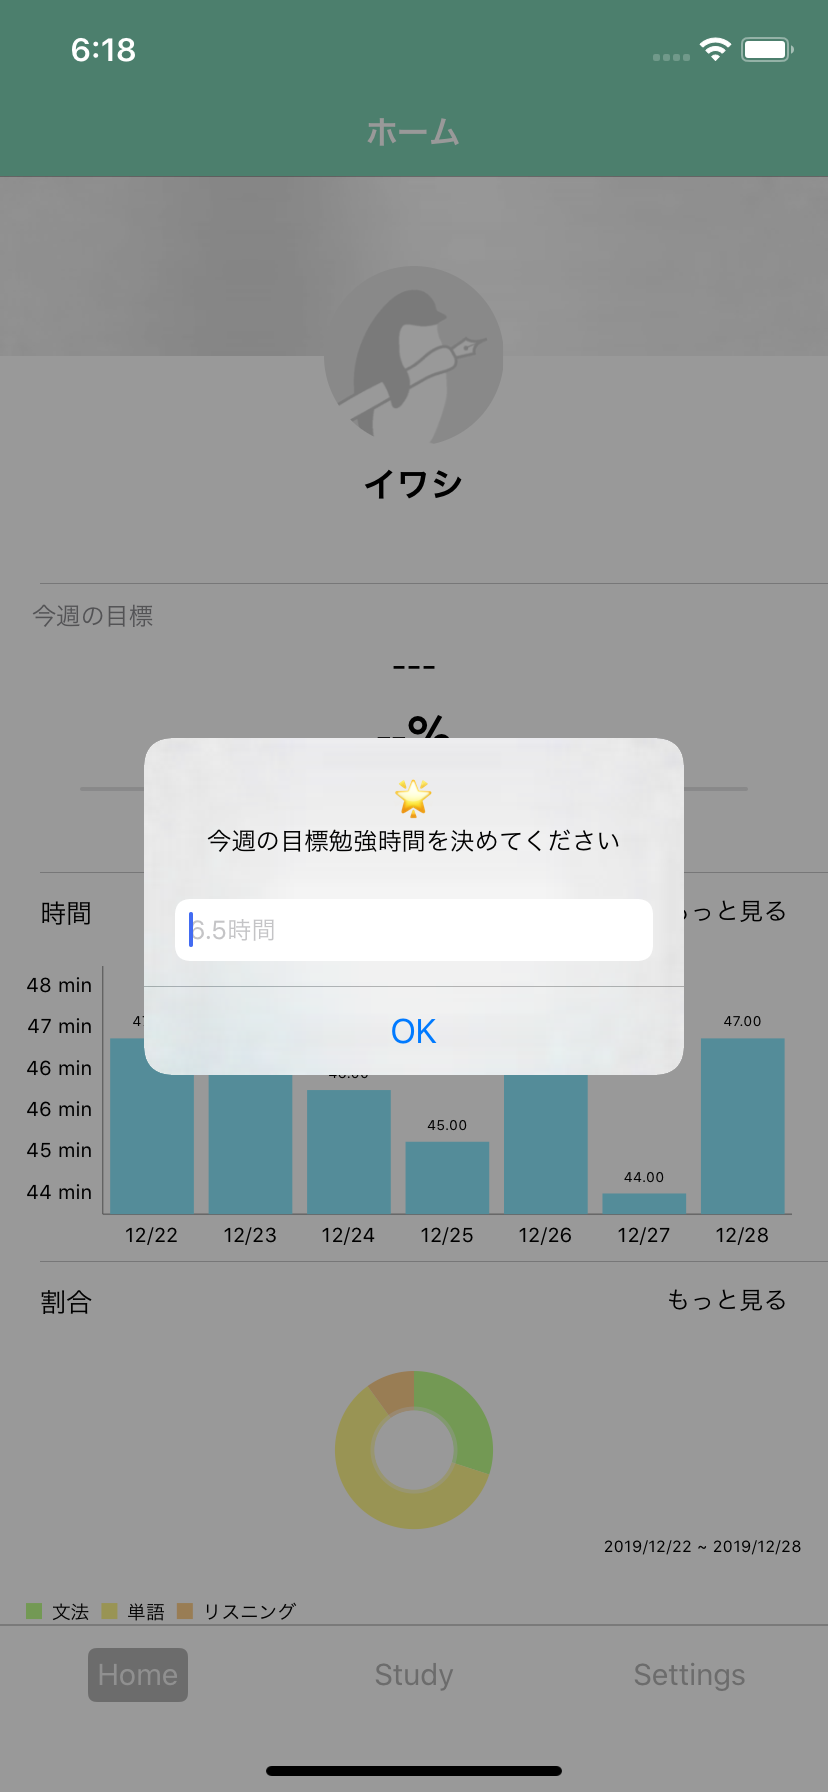
\includegraphics[width=5cm]{images/6/goal_alert.png}}
		\caption{目標設定アラート}
		\label{fig:goal_alert}
	\end{center}
  	\end{minipage}

  	\begin{minipage}[b]{0.5\linewidth}
	\begin{center}
		\fbox{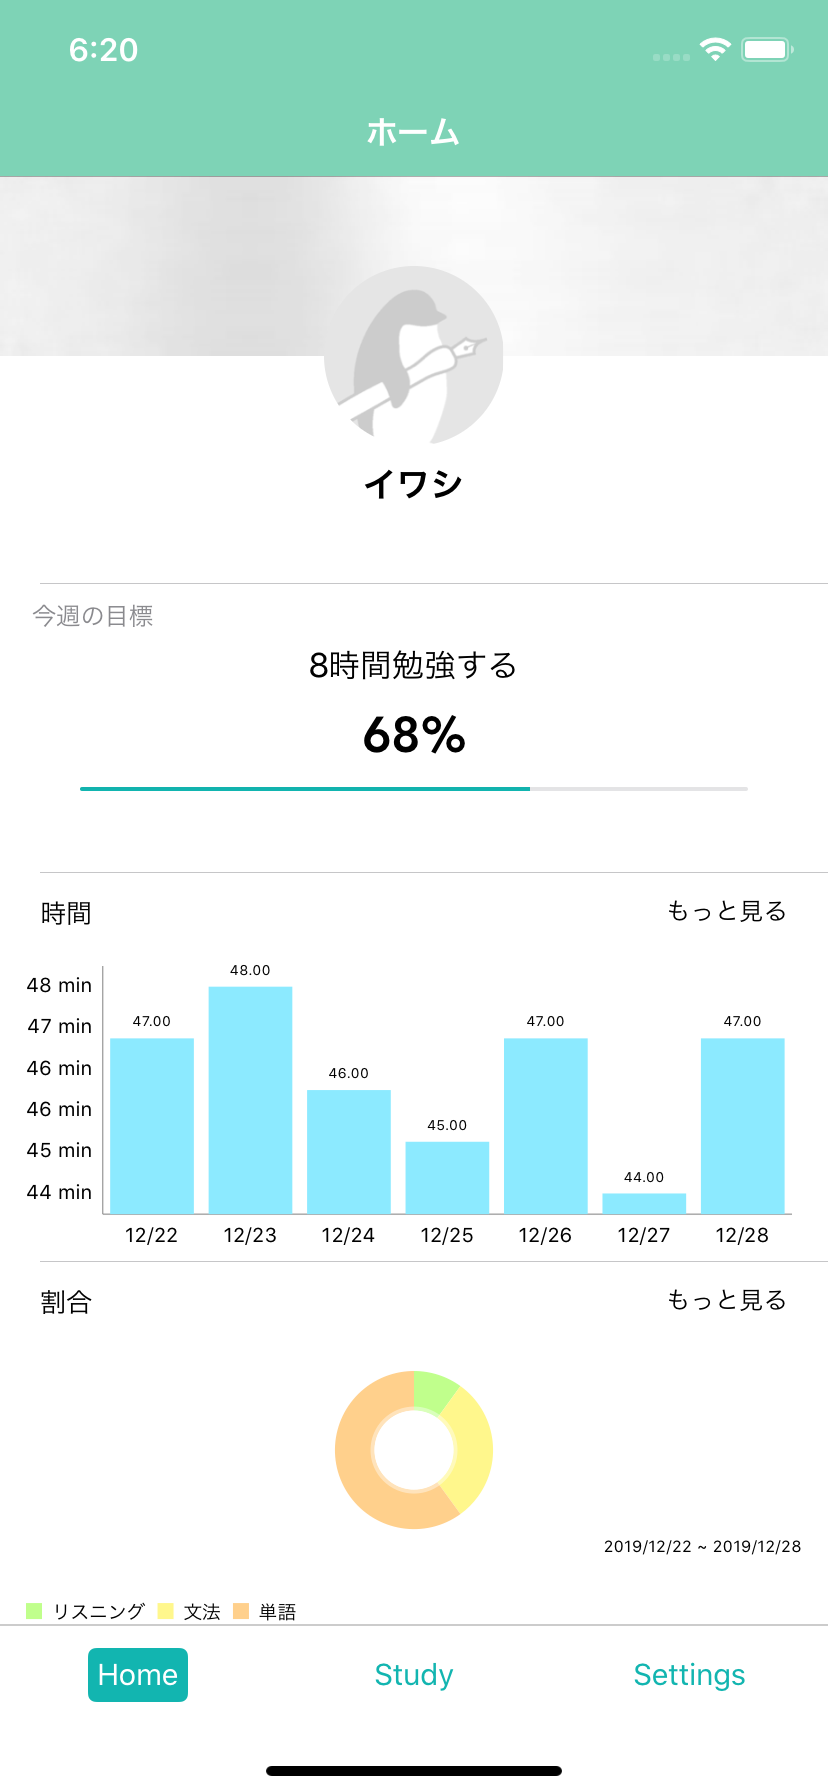
\includegraphics[width=5cm]{images/6/top_goal.png}}
		\caption{目標設定機能}
		\label{fig:top_goal}
	\end{center}
  	\end{minipage}

\end{tabular}
\end{center}
\end{figure}

\section{サーバ側実装}
サーバ及びデータベースには,MBaaSであるBack4App~\cite{back4app}を利用する.
データベースにはユーザの認証情報を格納するUserクラスと,ユーザ情報を格納するUserInformationObject, 学習記録を格納するStudyRecordObject, アンケート回答結果を格納するQuestionnaireObject, ユーザログを格納するLogObjectが存在する.
Userクラスの例を表~\ref{tb:user_class}に,UserInformationObjectの例を表~\ref{tb:user_information_object}に,StudyRecordObjectの例を表~\ref{tb:study_record_object}に,
QuestionnaireObjectの例を表~\ref{tb:questionnaire_object}に,LogObjectの例を表~\ref{tb:log_object}に示す.

\begin{table}[htb]
\begin{center}
  \begin{tabular}{|l|l|} \hline
    カラム名 & 値 \\ \hline
    objectId & ``1gGQysuNVu" \\
    username & ``test@test.com" \\
    password & ``dummypassword" \\
    ACL & ``1gGQysuNVu" \\
	createdAt & 2019-10-26T04:18:50.730Z \\
	updatedAt & 2019-10-26T04:18:50.730Z \\ \hline
  \end{tabular}
  \caption{Userクラスの例}
  \label{tb:user_class}
\end{center}
\end{table}

\begin{figure}[htb]
\begin{center}
\begin{tabular}{c}

\begin{minipage}[htb]{\linewidth}
\begin{center}
  \begin{tabular}{|l|l|} \hline
    カラム名 & 値 \\ \hline
    objectId & ``tDJeKhoeEF" \\
    userId & ``1gGQysuNVu" \\
    usernameForUser & ``アンコウ" \\
    userAim & ``" \\
    profileImageFile & 895ffca37d3e0f1efb4b347333fea8c6\_profileImage.png \\
    subject & [``数学", ``英語", ``国語", ``理科", ``社会"] \\
    content & [``予習", ``復習", ``課題", ``テスト勉強"] \\
    gender & ``unspecified" \\
    birthday & null \\
    buildVersion & 6 \\
	createdAt & 2019-10-26T04:18:50.730Z \\
	updatedAt & 2019-10-26T04:18:50.730Z \\ \hline
  \end{tabular}
  \caption{UserInformationObjectの例}
  \label{tb:user_information_object}
\end{center}
\end{minipage}

\\

\begin{minipage}[htb]{0.5\linewidth}
\begin{center}
  \begin{tabular}{|l|l|} \hline
    カラム名 & 値 \\ \hline
    objectId & ``cYYmKJ6b4U" \\
    user & PFUser(``1gGQysuNVu") \\
    subject & ``英語" \\ 
    content & ``文法" \\ 
	studyTime & 3600 \\ 
	isInterruption & false \\ 
	byHand & true \\  
	studyDate & 2019-11-04T15:00:00.000Z \\
	createdAt & 2019-11-05T07:24:08.810Z \\
	updatedAt & 2019-11-05T07:24:08.810Z \\ \hline
  \end{tabular}
  \caption{StudyRecordObjectの例}
  \label{tb:study_record_object}
\end{center}
\end{minipage}

\begin{minipage}[htb]{0.5\linewidth}
\begin{center}
  \begin{tabular}{|l|l|} \hline
    カラム名 & 値 \\ \hline
    objectId & ``JUaSnsWBqy" \\
    user & PFUser(``1gGQysuNVu") \\
    score & [9, 10, 12, 11] \\
    motivation & ``Identified" \\
    feature & ``Goal" \\
	createdAt & 2019-10-31T22:46:27.983Z \\
	updatedAt & 2019-10-31T22:46:27.983Z \\ \hline
  \end{tabular}
  \caption{QuestionnaireObjectの例}
  \label{tb:questionnaire_object}
\end{center}
\end{minipage}

\\

\begin{minipage}[htb]{\linewidth}
\begin{center}
  \begin{tabular}{|l|l|} \hline
    カラム名 & 値 \\ \hline
    objectId & ``gcpDfzEl1u" \\
    user & PFUser(``1gGQysuNVu") \\
    eventName & ``appOpen" \\
	createdAt & 2019-10-26T05:20:14.594Z \\
	updatedAt & 2019-10-26T05:20:14.594Z \\ \hline
  \end{tabular}
  \caption{LogObjectの例}
  \label{tb:log_object}
\end{center}
\end{minipage}

\end{tabular}
\end{center}
\end{figure}


\section{まとめ}
本章では,Stuguinシステムの実装について述べた.
次章では,本システムで得られたデータから動機づけの向上を評価し,考察について述べる.
